






We discuss in this section the robustness of our results.\\
We first show that the backlash phenomenon that we measure is consistent between French geographical regions. To do so, we re-estimate our preferred specification on a series of sub-samples in which we sequentially exclude each broad region from the analysis. We display these results in \autoref{fig:by_region}. Dropping the regions in the North of France, the estimated backlash effect becomes larger in magnitude. This is consistent with the fact that Northern camps were, on average, less visible, of a smaller size and generated fewer local tensions. It is also consistent with the difference in the composition of the hosted population: Northern camps and centres welcome a higher share of women and children, which plausibly reduces the magnitude of the backlash effect we measure. Consistently, when we exclude regions in the South, the estimated coefficient moves towards zero and the implied backlash is smaller, in line with the idea that camps in the South were more visible and politically salient. The pattern of our results is nevertheless preserved across all leave-one-out specifications: the sign of the estimated effect remains unchanged. Overall, this suggests that no single region is driving our main results.

\begin{figure}[htbp]
  \centering
  \caption{Effect on socialist vote share - Leave one out results}
  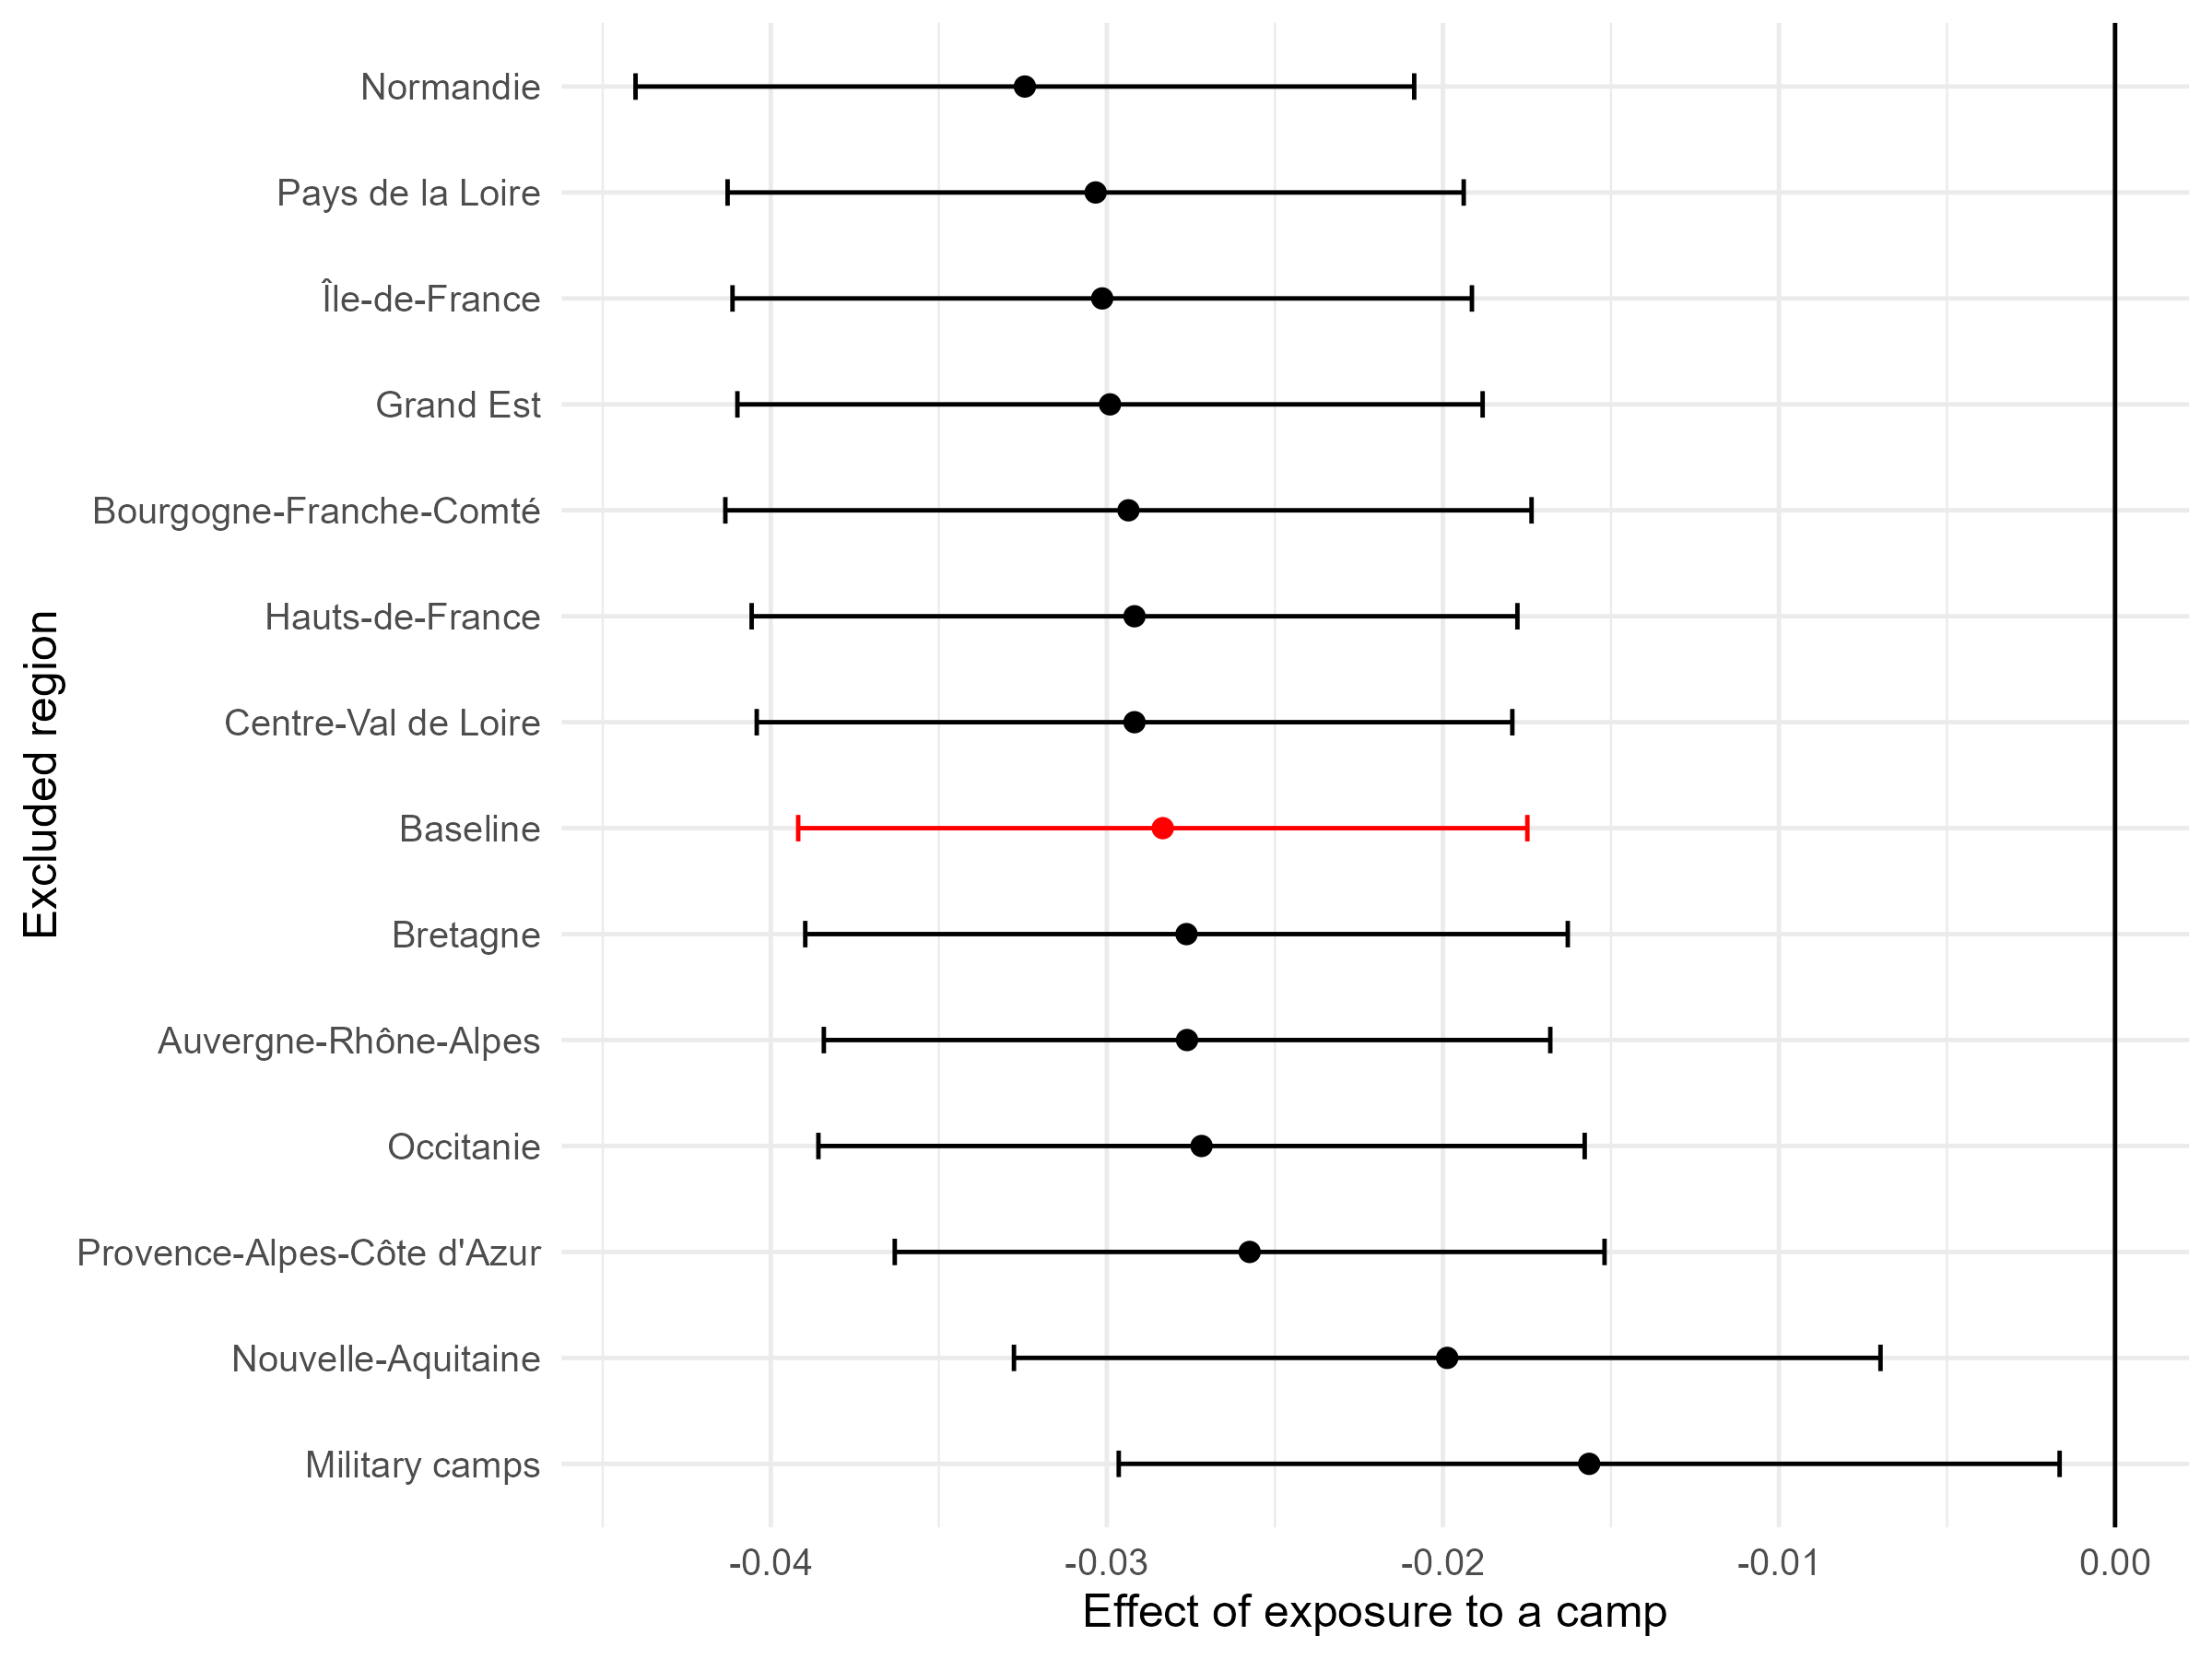
\includegraphics[width=0.6\linewidth]{../figures/results/political/by_region_sfio.png}
  \label{fig:by_region}
   \begin{minipage}{0.7\textwidth}
   \vspace{0.1in} 
        {\tiny Notes: This graph reports the estimates leaving one region out at the time of the baseline TWFE. Error bars plot the interval confidence at 95\%. Standard errors are clustered at the municipal level.\par}
        \end{minipage}
\end{figure}

\begin{figure}[htbp]
  \centering
  \caption{Effect on communist vote share - Leave one out results}
  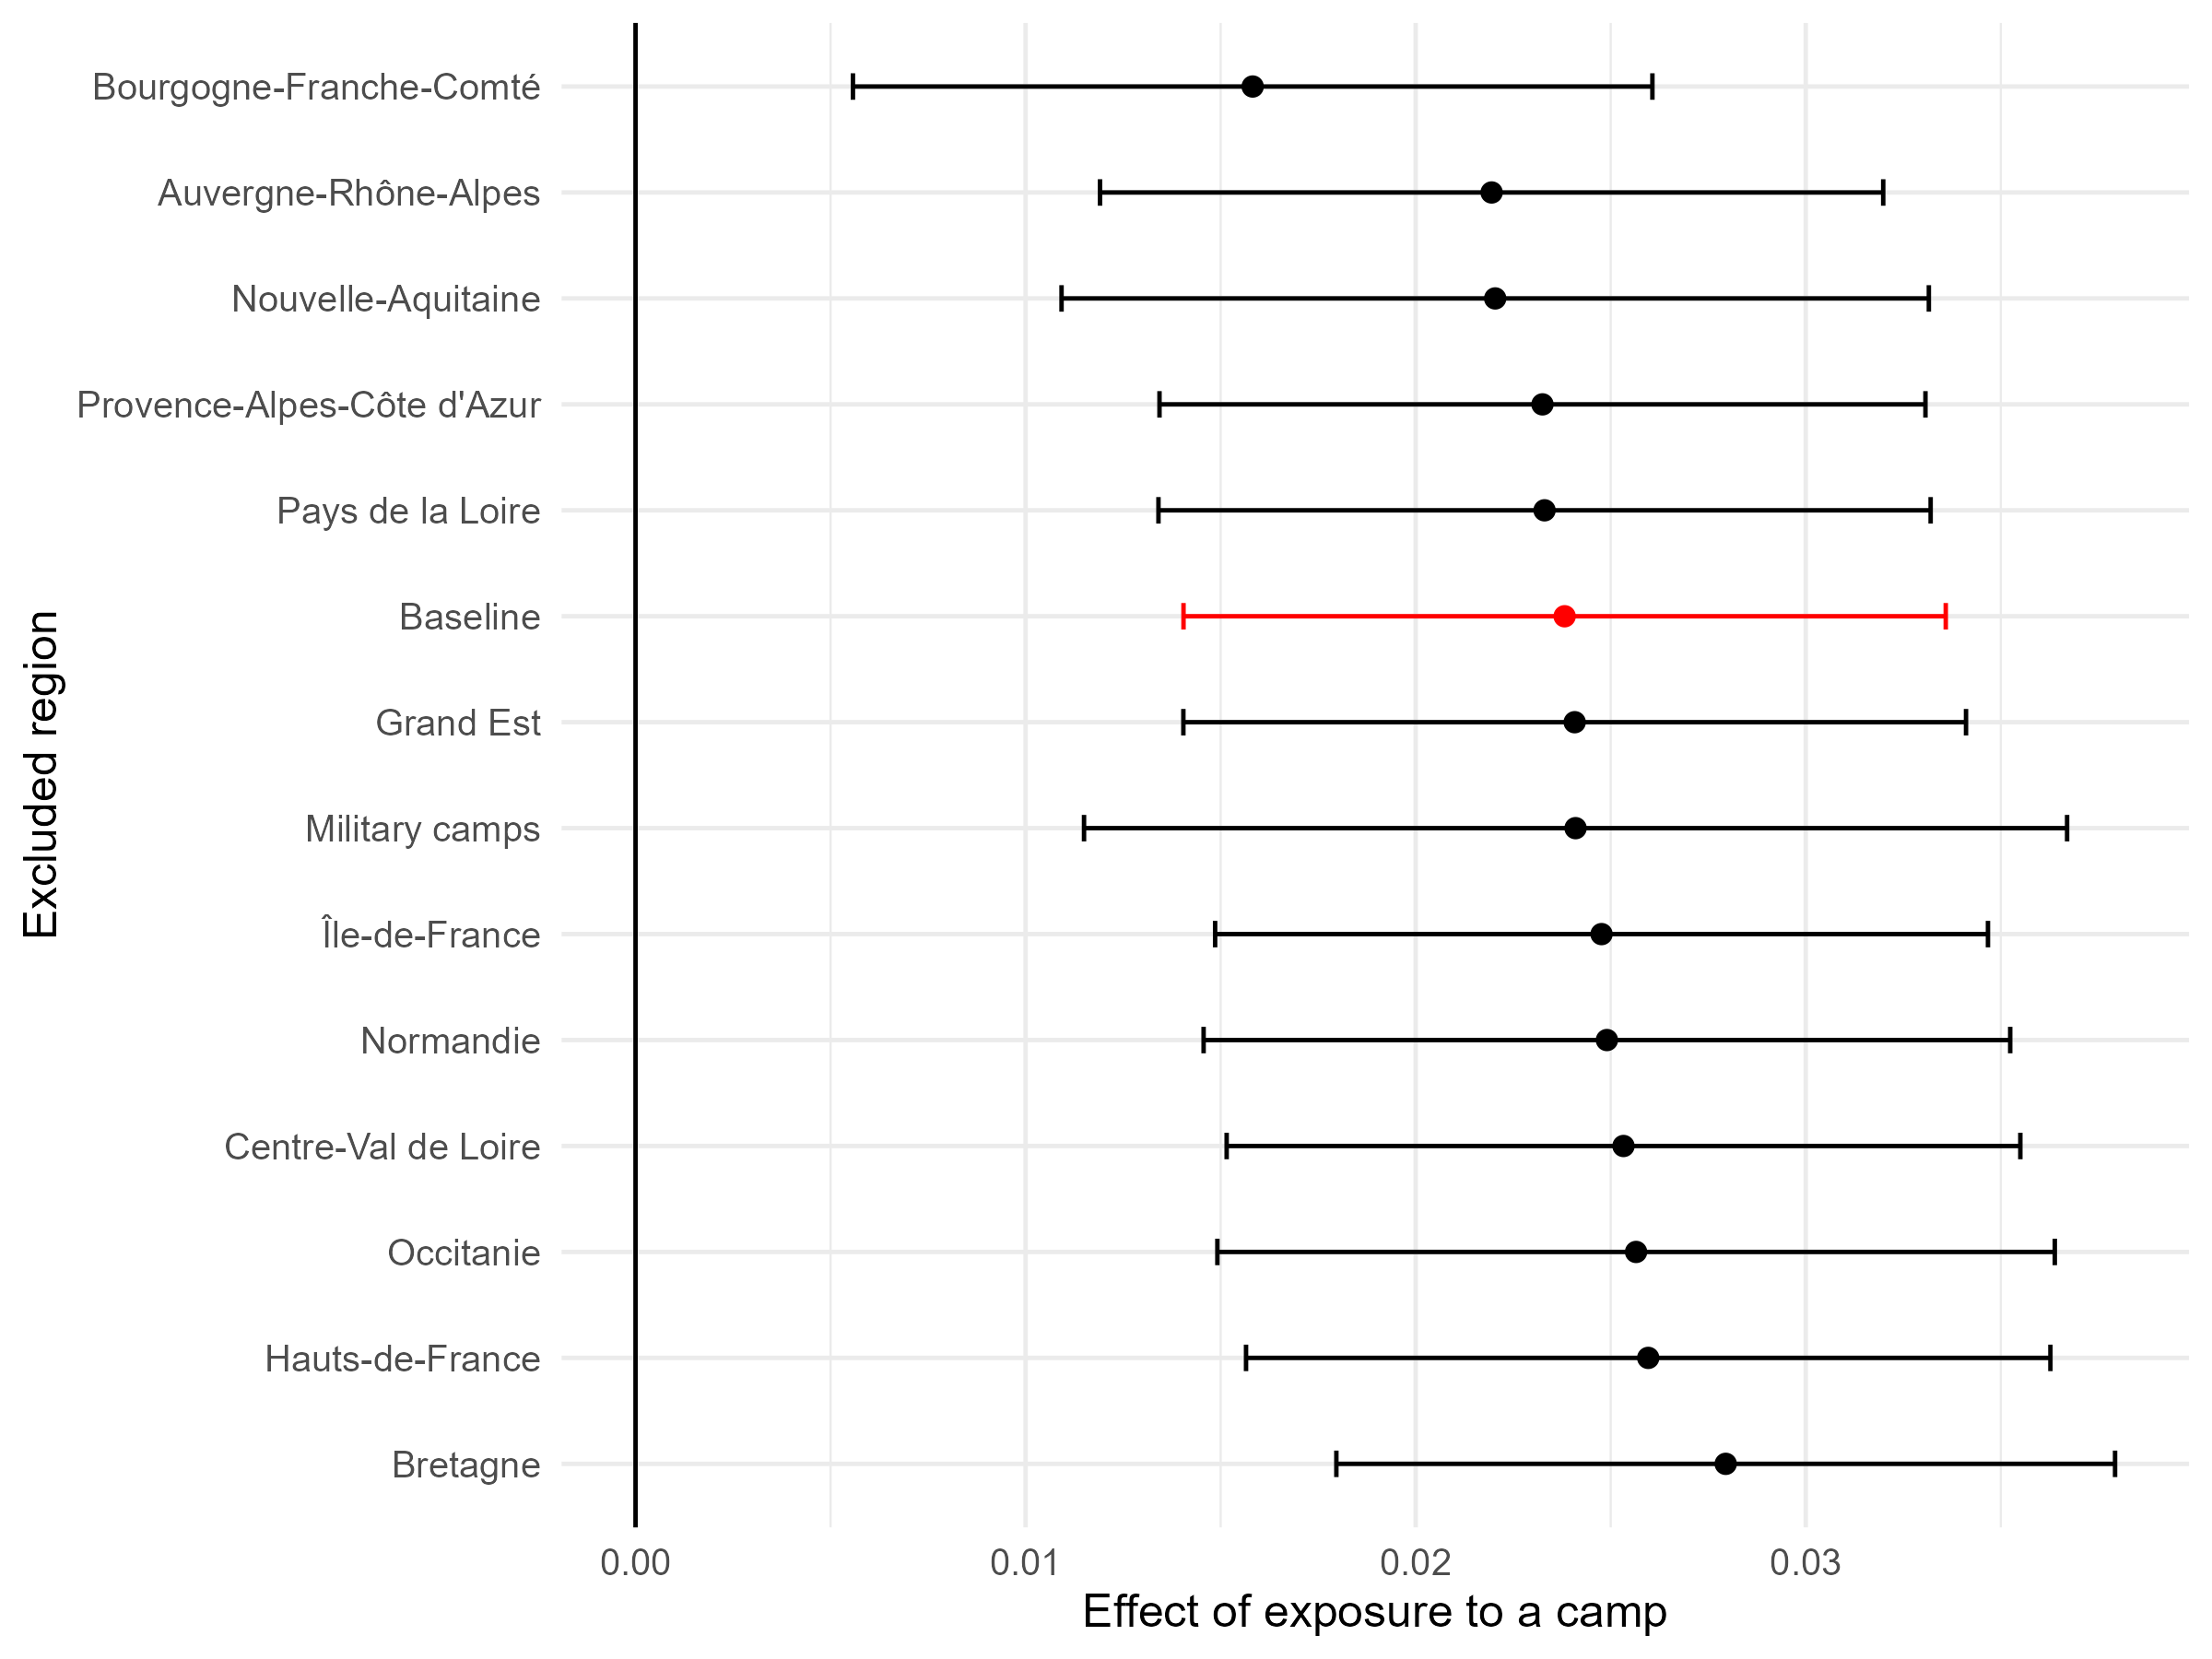
\includegraphics[width=0.6\linewidth]{../figures/results/political/by_region_pcf.png}
  \label{fig:by_region}
   \begin{minipage}{0.7\textwidth}
   \vspace{0.1in} 
        {\tiny Notes: This graph reports the estimates leaving one region out at the time of the baseline TWFE. Error bars plot the interval confidence at 95\%. Standard errors are clustered at the municipal level.\par}
        \end{minipage}
\end{figure}

Similarly, we verify that our results are not driven by differential dynamics between the part of the country occupied by the German forces (\textit{zone occupée}) and the municipalities under the authority of the Vichy government (\textit{zone libre}). Exploiting this historical division also allows us to use occupation status as a proxy for the local intensity of the Second World War and to check whether our estimates are simply capturing the areas most directly affected by the conflict.

In order to do so, we re-estimate our baseline specification separately for municipalities located in the occupied and in the non-occupied zones. \autoref{fig:occupied} shows the results. Trends between treated and control municipalities are similar when we restrict the sample to the occupied zone and when we restrict it to the non-occupied zone, indicating that our main findings are not specific to one side of the demarcation line. If anything, the estimated backlash is of a larger magnitude in the non-occupied areas, where the largest camps and soldiers refugee settlements are located. If the intensity of the war were driving our results, one would instead expect stronger effects in the occupied zone. This pattern reinforces the interpretation that our estimates capture a backlash mechanism linked to the presence of the camps rather than to wartime violence.

\begin{figure}[htbp]
  \centering
  \caption{Effect on socialist vote share - Occupied vs Non-Occupied areas}
  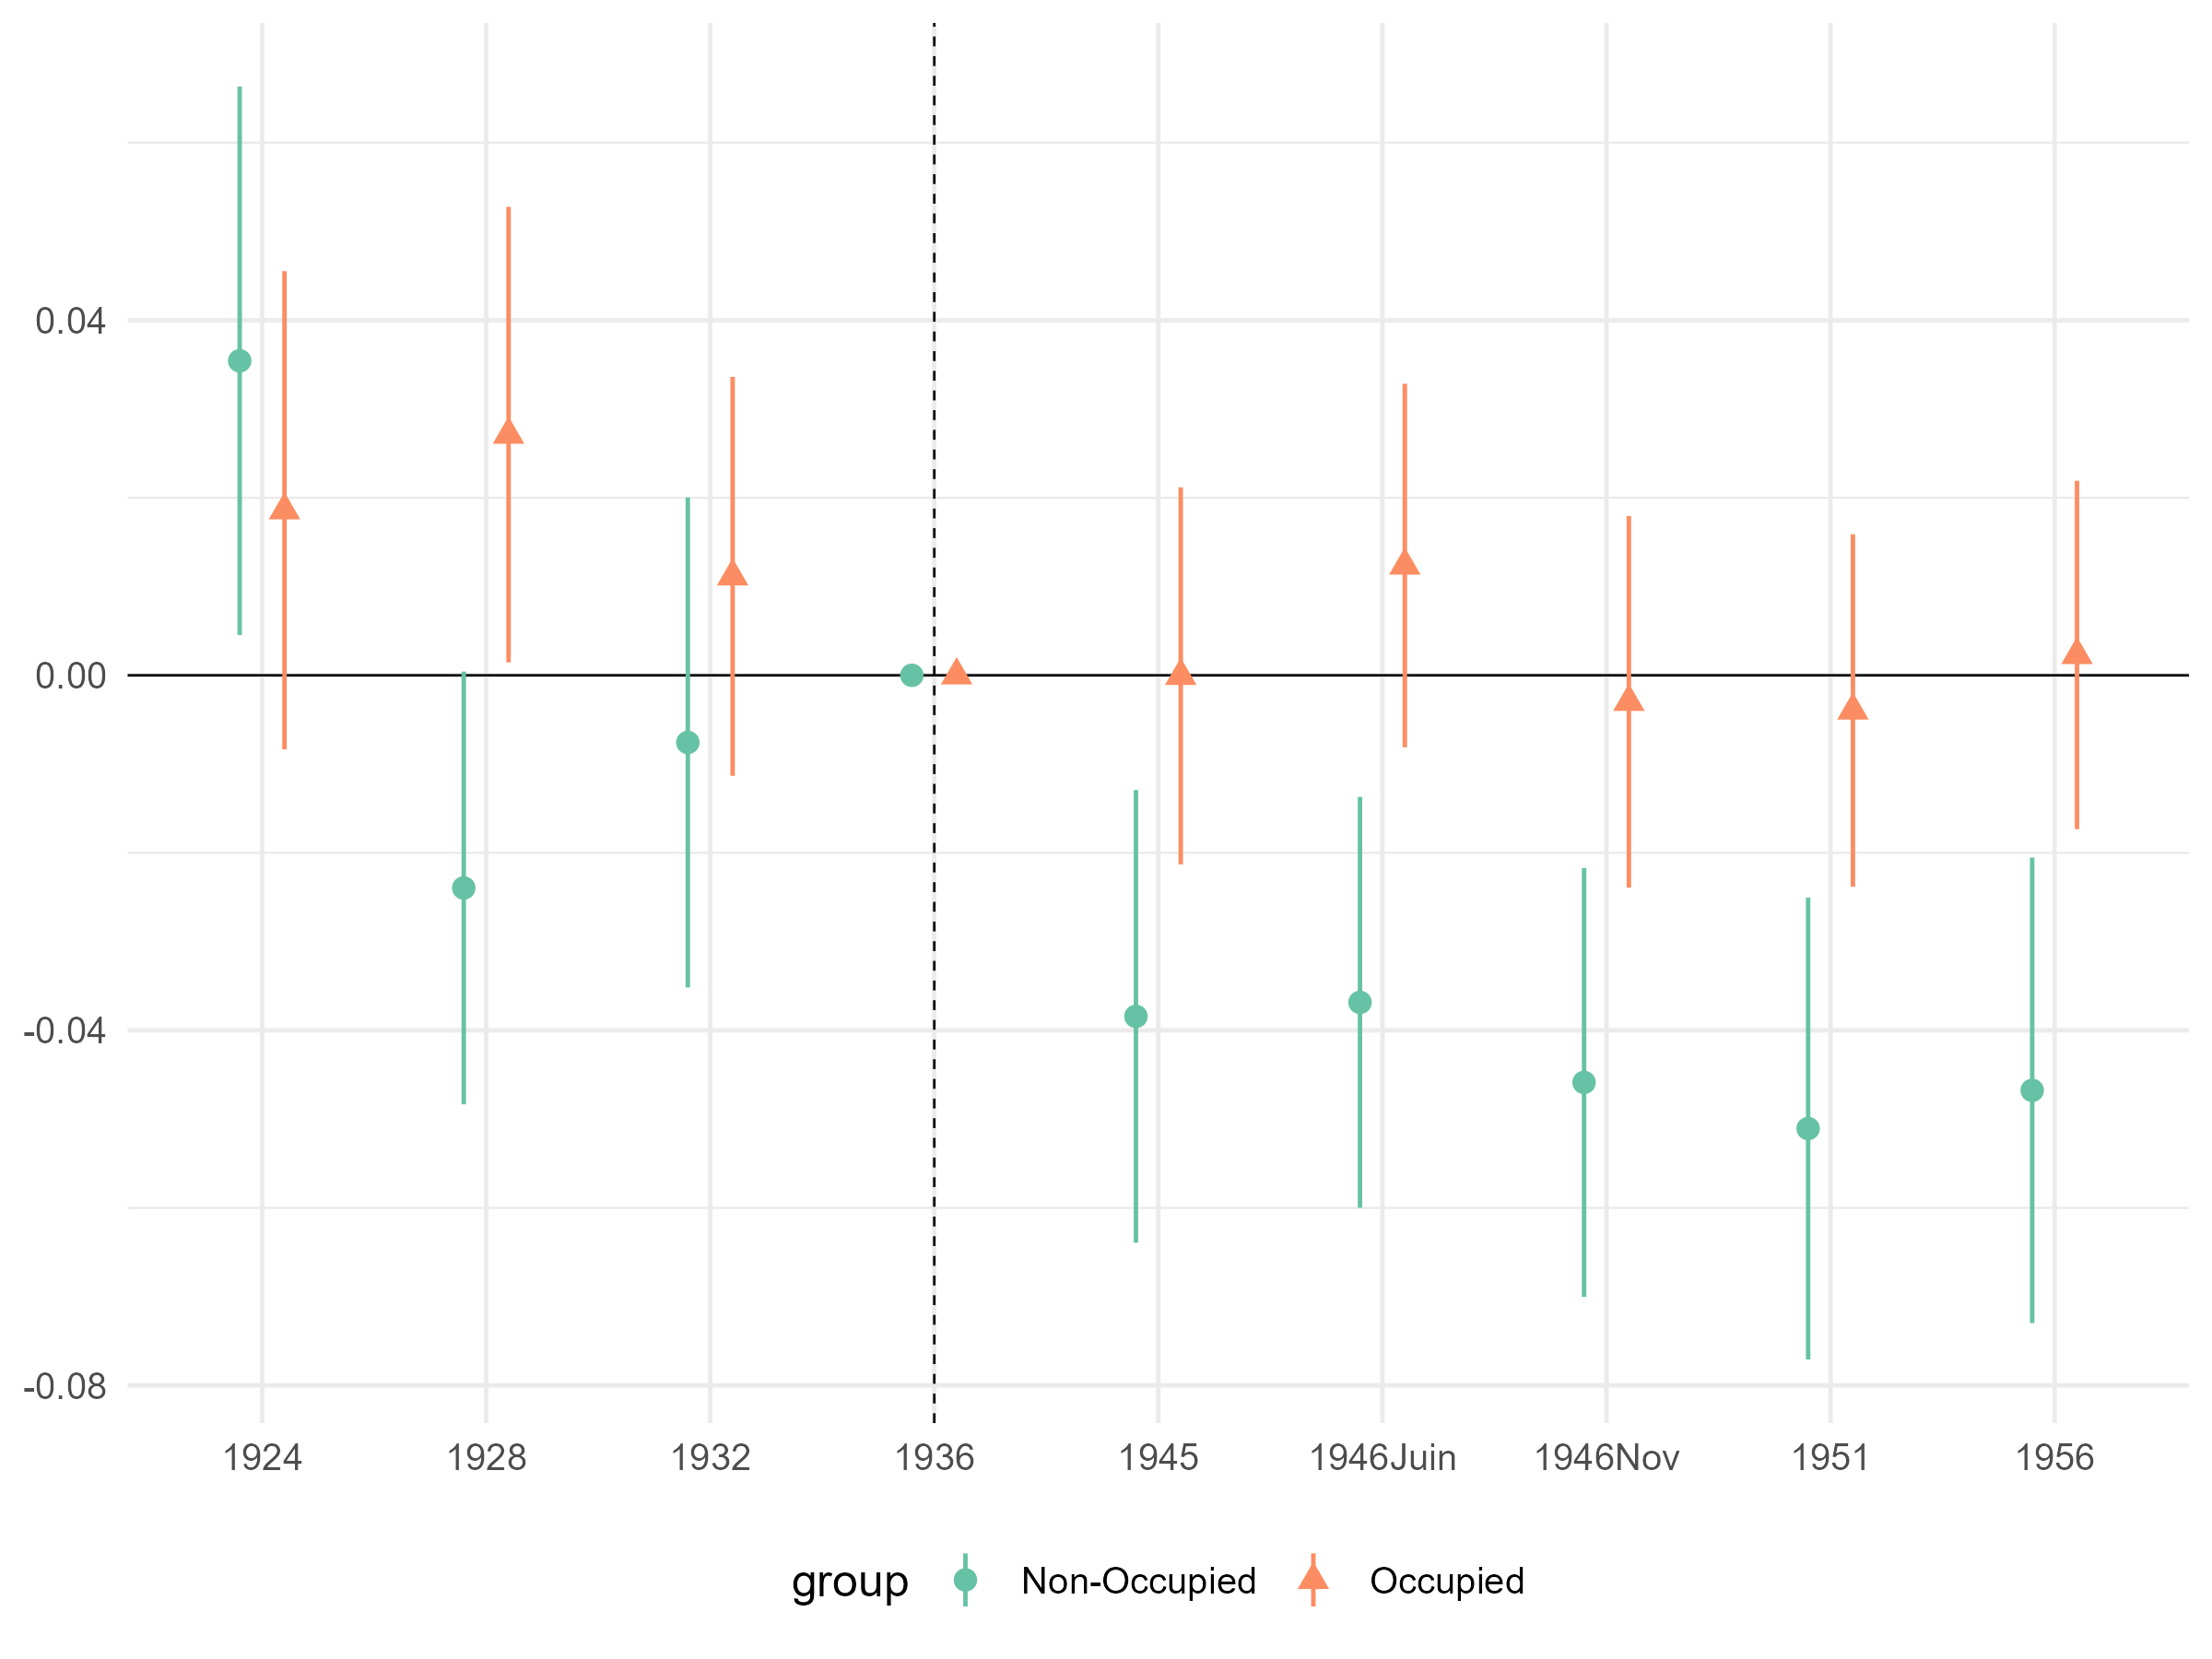
\includegraphics[width=0.7\linewidth]{../figures/results/political/occupied_sfio.png}
  \label{fig:occupied}
    \begin{minipage}{0.7\textwidth}
   \vspace{0.1in} 
   {\tiny Notes: This figure reports difference-in-differences estimates separately for the Nazi-occupied zone and the non-occupied Vichy zone. Error bars show 95\% confidence intervals. Standard errors are clustered at the municipality level.\par}
        \end{minipage}
\end{figure}

\begin{figure}[htbp]
  \centering
  \caption{Effect on communist vote share - Occupied vs Non-Occupied areas}
  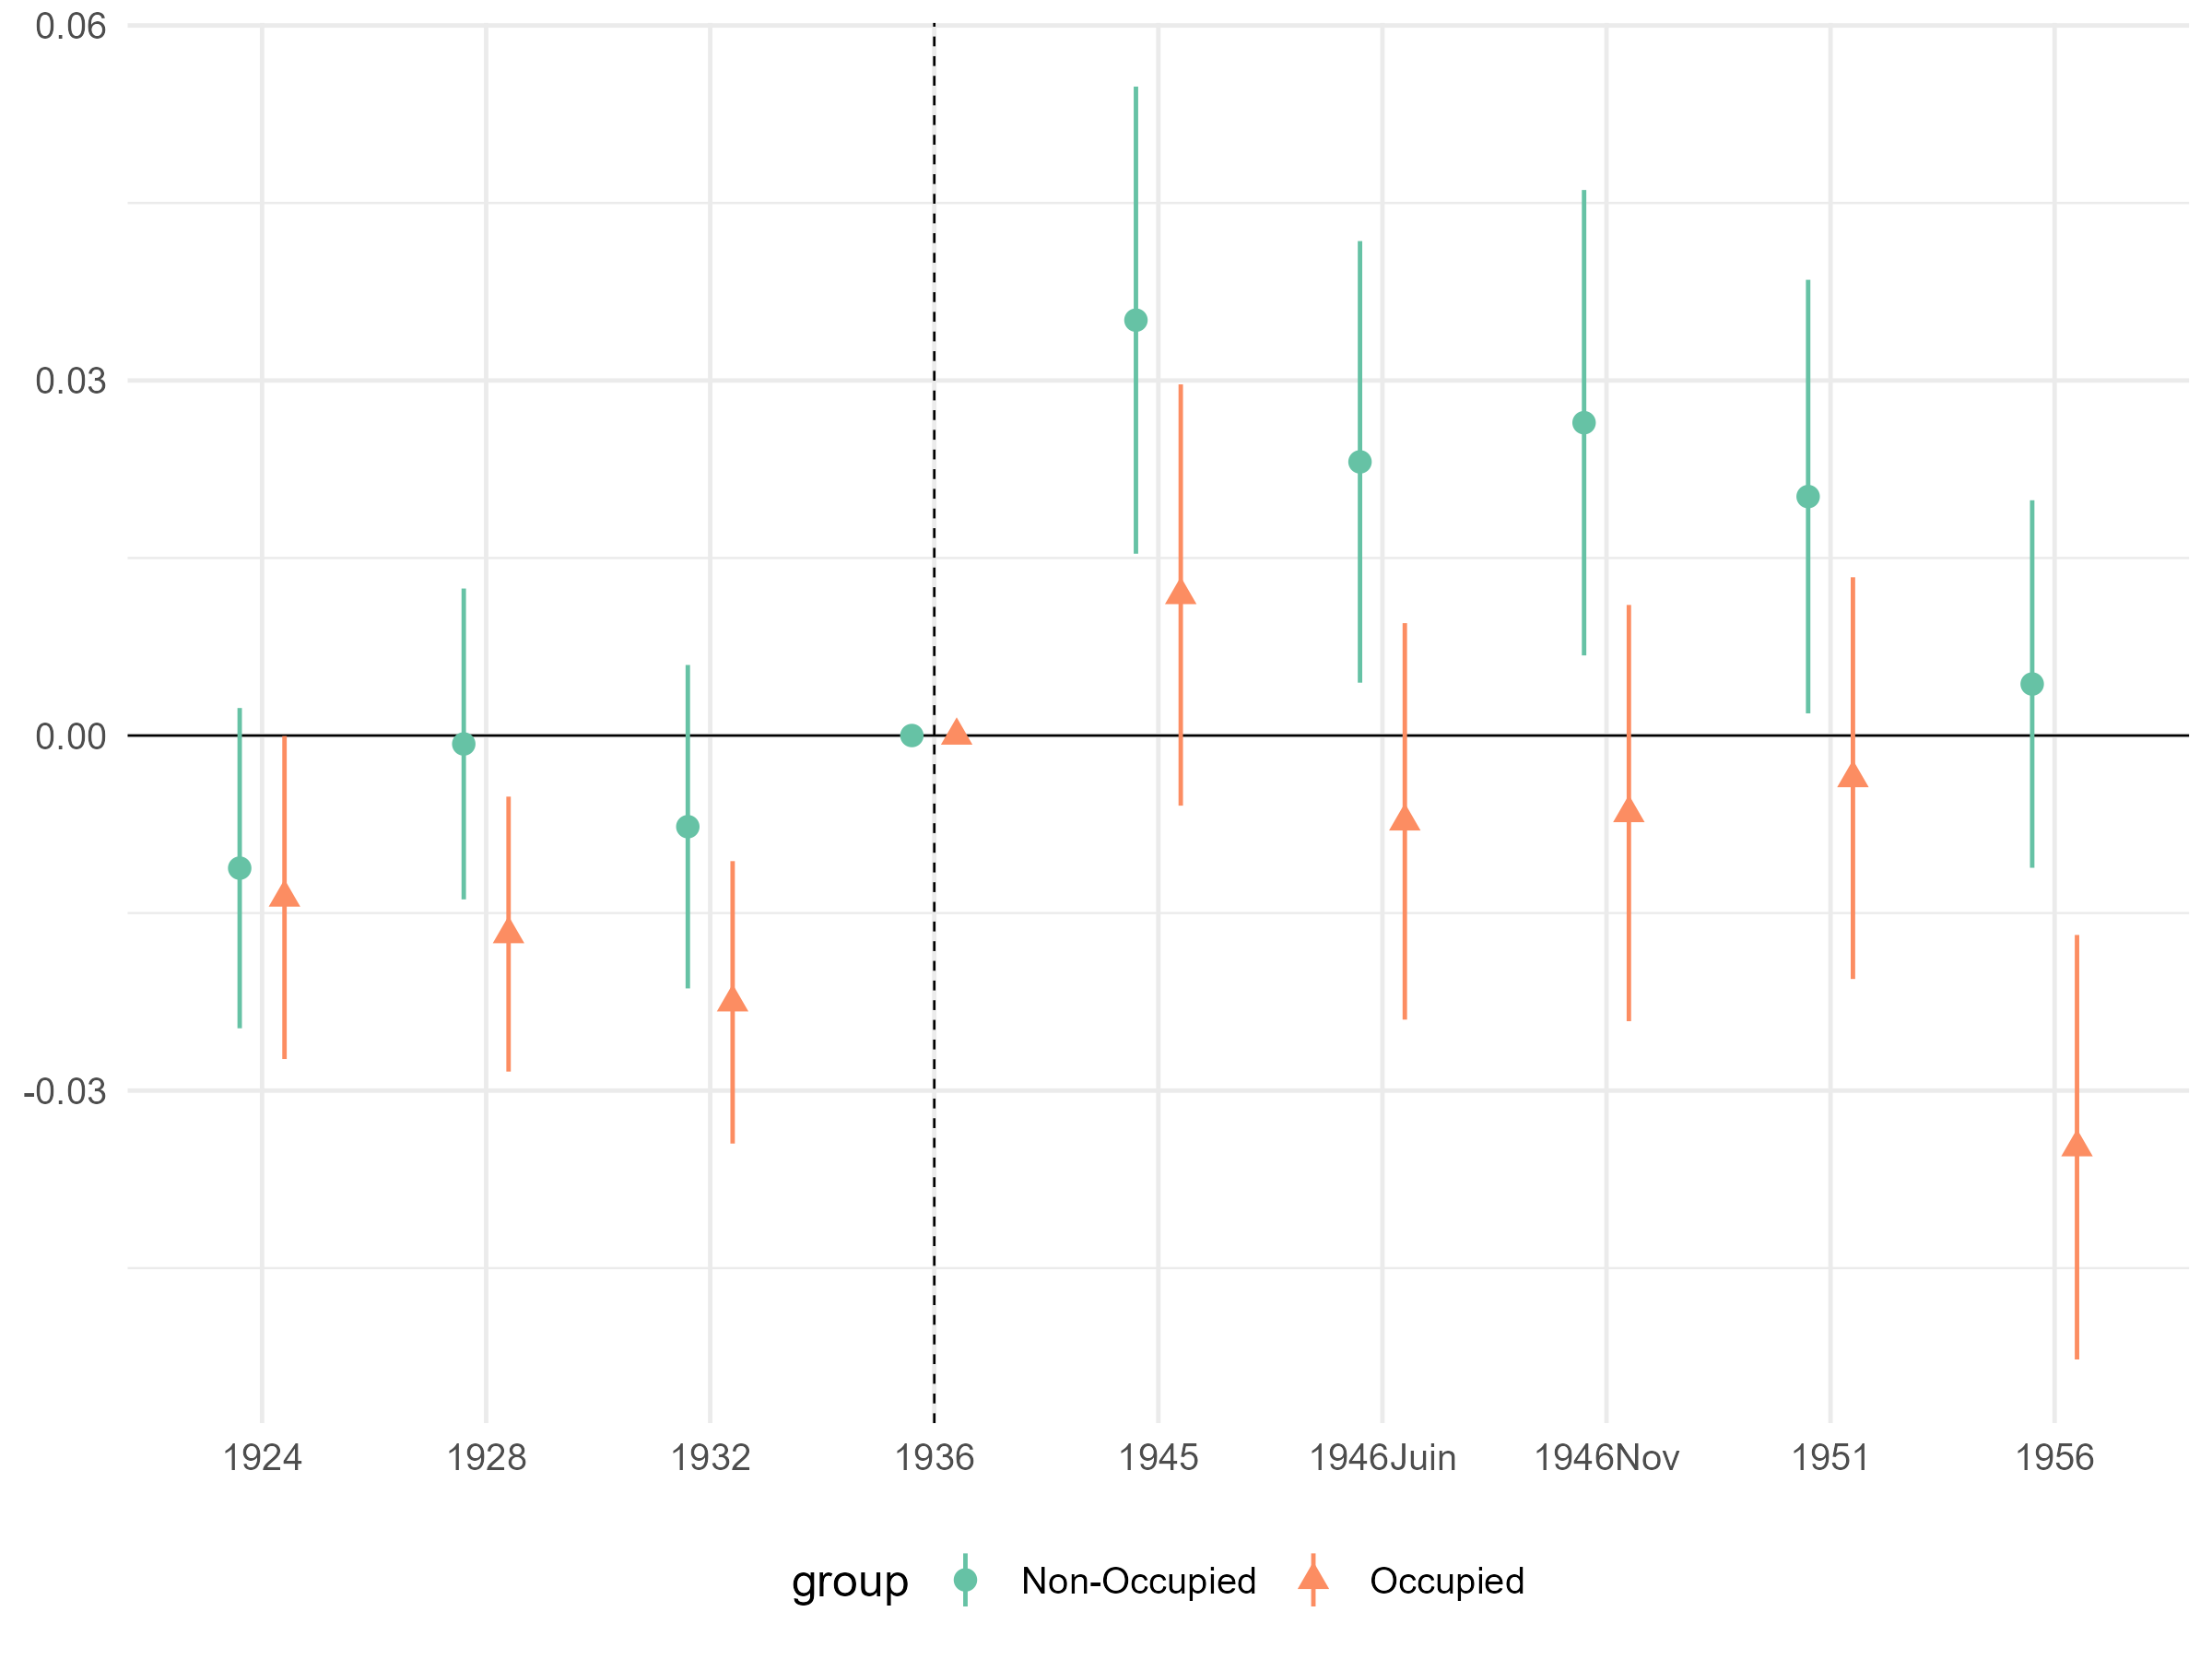
\includegraphics[width=0.7\linewidth]{../figures/results/political/occupied_pcf.png}
  \label{fig:occupied}
    \begin{minipage}{0.7\textwidth}
   \vspace{0.1in} 
   {\tiny Notes: This figure reports difference-in-differences estimates separately for the Nazi-occupied zone and the non-occupied Vichy zone. Error bars show 95\% confidence intervals. Standard errors are clustered at the municipality level.\par}
        \end{minipage}
\end{figure}

SYNTHETIC DID 

\begin{table}[h!]
    \centering
    \caption{Impact of refugee camp exposure on the vote shares - Synthetic DiD}
    \resizebox{0.4\textwidth}{!}{\begin{tabular}{lcccc}
\toprule
 & \multicolumn{2}{c}{\textit{SFIO Vote Share}} & \multicolumn{2}{c}{\textit{PCF Vote Share}} \\
\cmidrule(lr){2-3}\cmidrule(lr){4-5}
 & (1) SDID & (2) SDID + Cov. & (1) SDID & (2) SDID + Cov. \\
\midrule
Within 1 km & -0.0328*** & -0.0314*** & 0.0287*** & 0.0285*** \\
 & (0.0033) & (0.0066) & (0.0037) & (0.0023) \\
Ring 5--10 km & -0.0232*** & -0.0232*** & 0.0289*** & 0.0287*** \\
 & (0.0024) & (0.0019) & (0.0041) & (0.0023) \\
Ring 10--15 km & -0.0205** & -0.0206*** & 0.0197*** & 0.0194*** \\
 & (0.0096) & (0.0033) & (0.0049) & (0.0013) \\
Ring 15--20 km & -0.0176*** & -0.0177*** & 0.0149*** & 0.0148*** \\
 & (0.0022) & (0.0007) & (0.0020) & (0.0017) \\
Ring 20--25 km & -0.0118*** & -0.0118*** & 0.0086*** & 0.0083*** \\
 & (0.0033) & (0.0015) & (0.0013) & (0.0025) \\
Ring 30--35 km & 0.0042 & 0.0047 & -0.0019 & -0.0022 \\
 & (0.0039) & (0.0029) & (0.0024) & (0.0018) \\
\bottomrule
\multicolumn{5}{l}{\footnotesize Standard errors in parentheses. $^{*}p<0.10$, $^{**}p<0.05$, $^{***}p<0.01$} \\
\end{tabular}
}
    \label{table:table_synthetic}
    \par
        \begin{minipage}{0.4\textwidth}
        \vspace{0.5em}
            \footnotesize
            Note: The table reports the synthetic DiD estimates of being located within a given distance ring from the refugee camps. The control group are those within 20-40km.  Standard errors (SE) are obtained using the placebo procedure. *** p$<$0.01, ** p$<$0.05, * p$<$0.1.
        \end{minipage}
\end{table}

\begin{figure}[htbp]
  \centering
  \caption{Effect on socialist vote share - Comparative between DiD and synthetic DiD}
  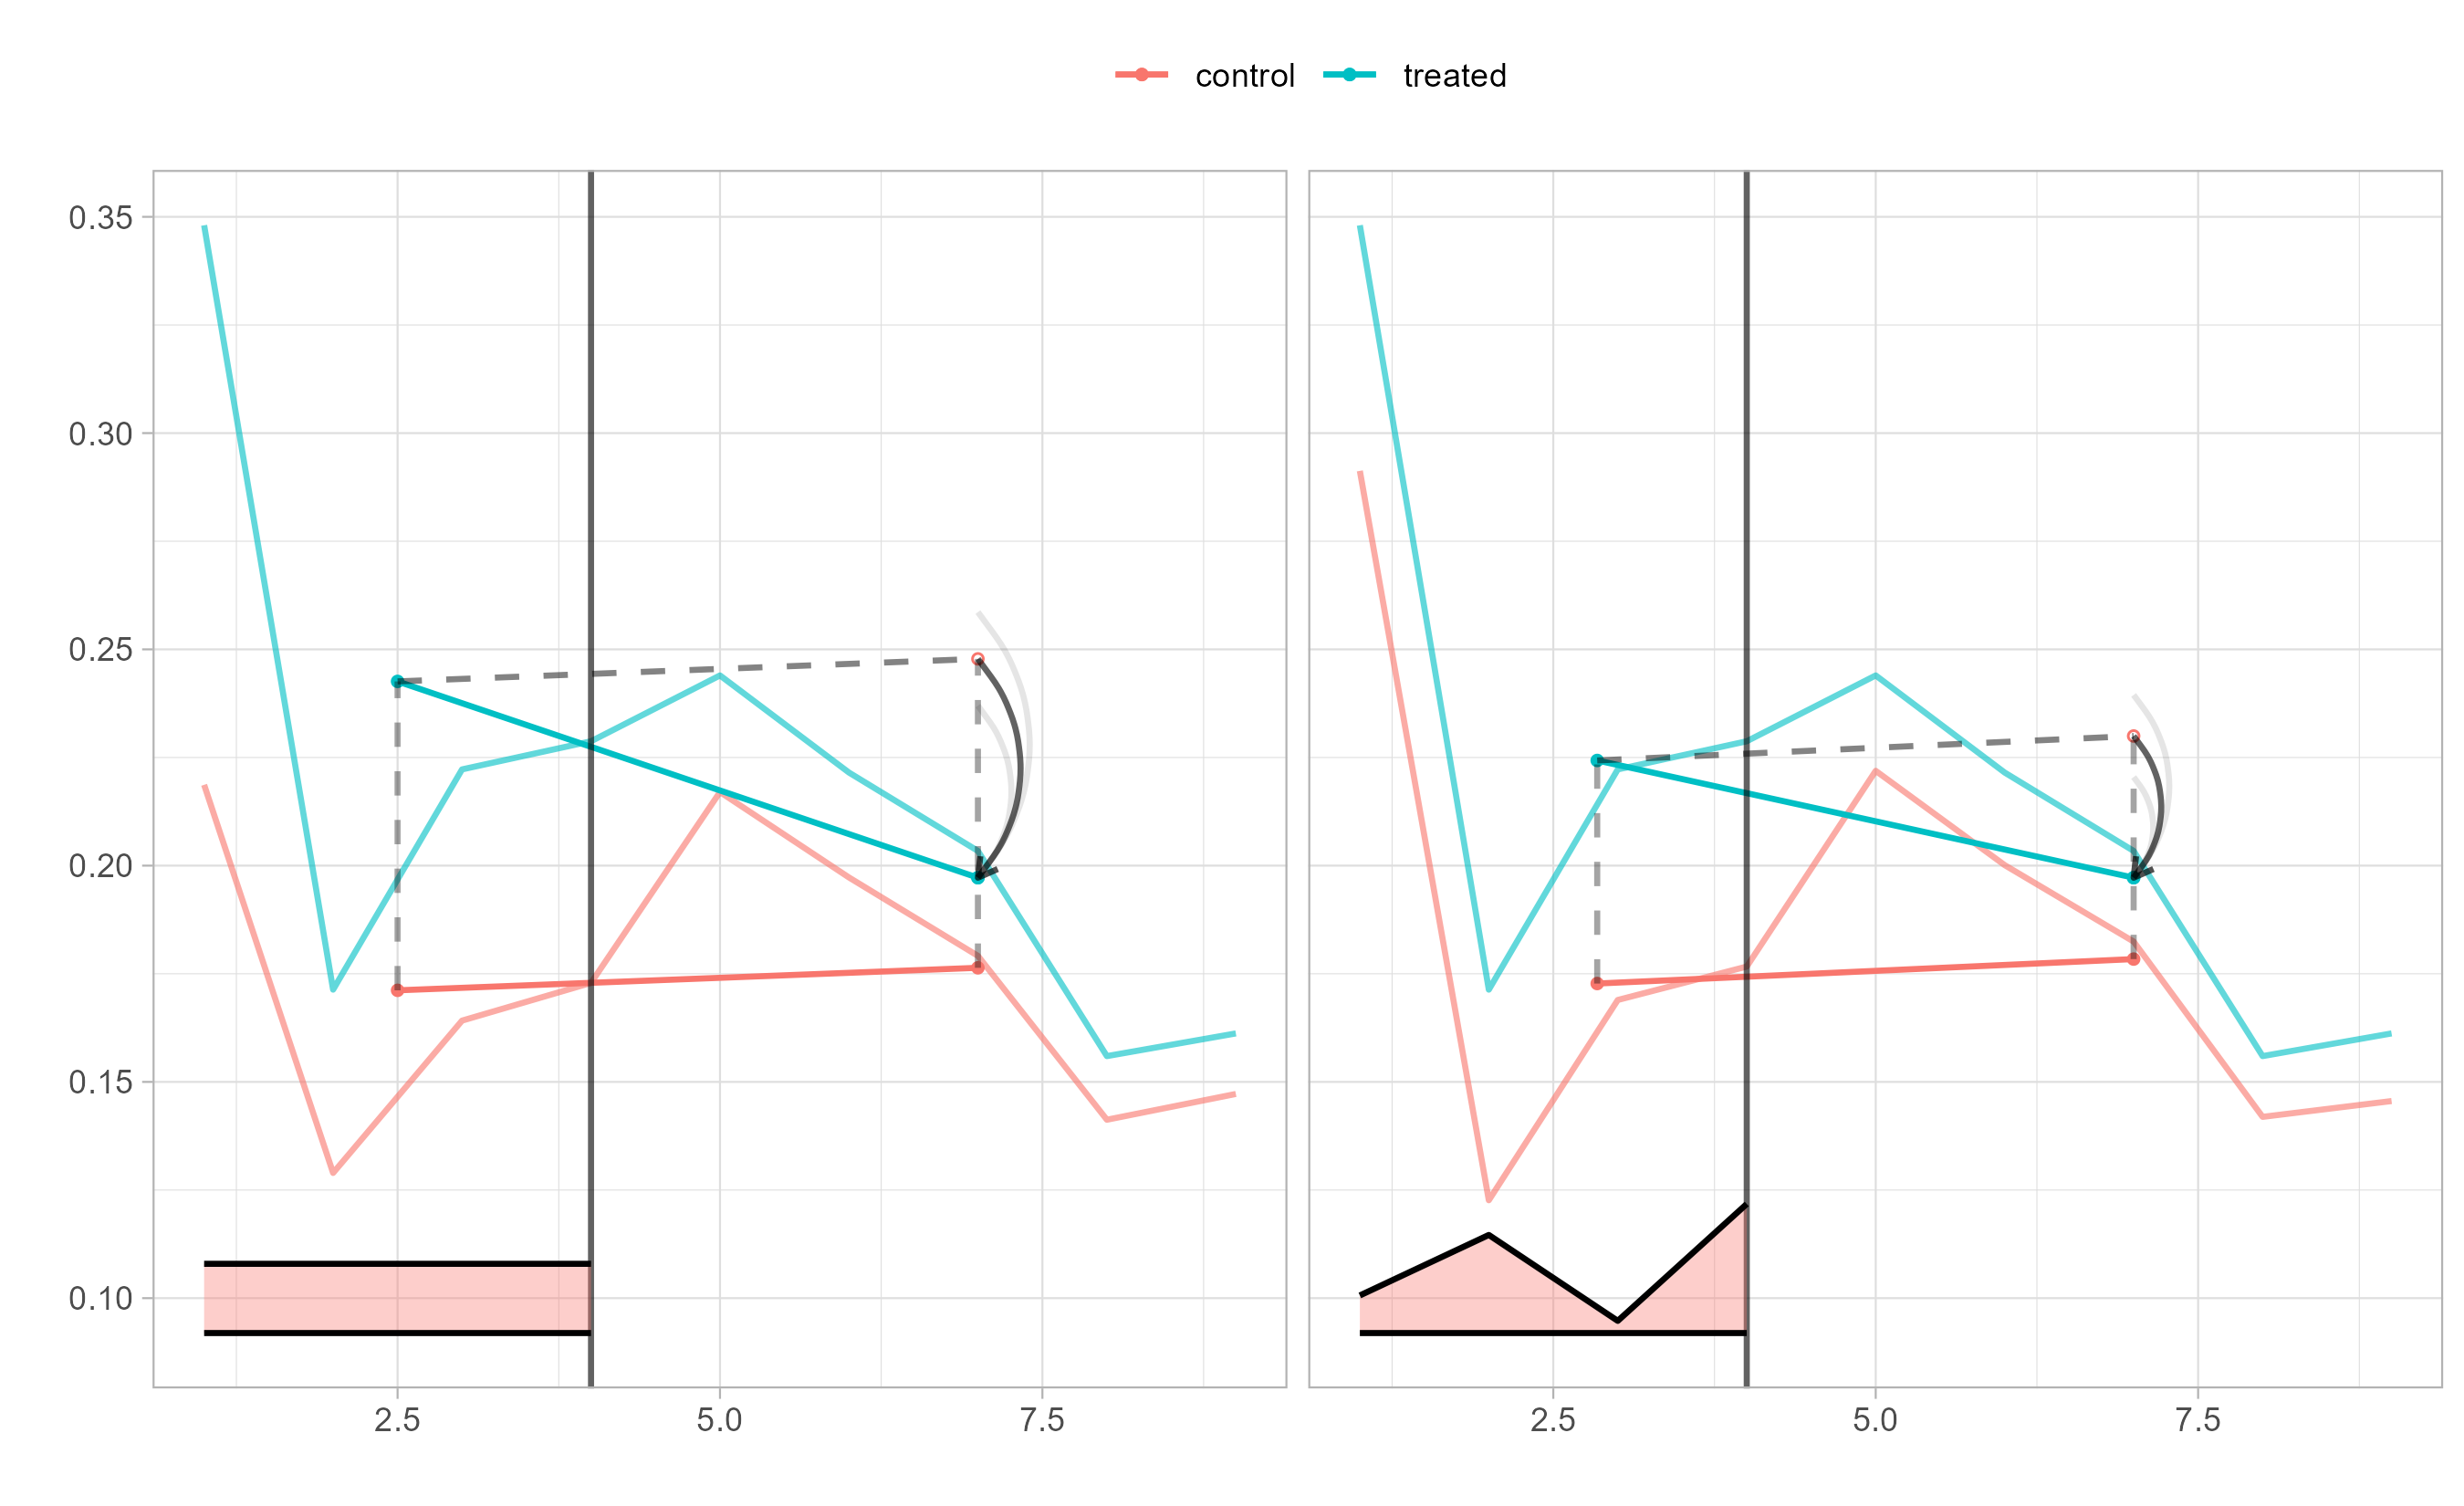
\includegraphics[width=0.7\linewidth]{../figures/results/political/comparison_sfio.png}
  \label{fig:comparison}
    \begin{minipage}{0.7\textwidth}
   \vspace{0.1in} 
   {\tiny Notes: .\par}
        \end{minipage}
\end{figure}


\begin{figure}[htbp]
  \centering
  \caption{Effect on communist vote share - Comparative between DiD and synthetic DiD}
  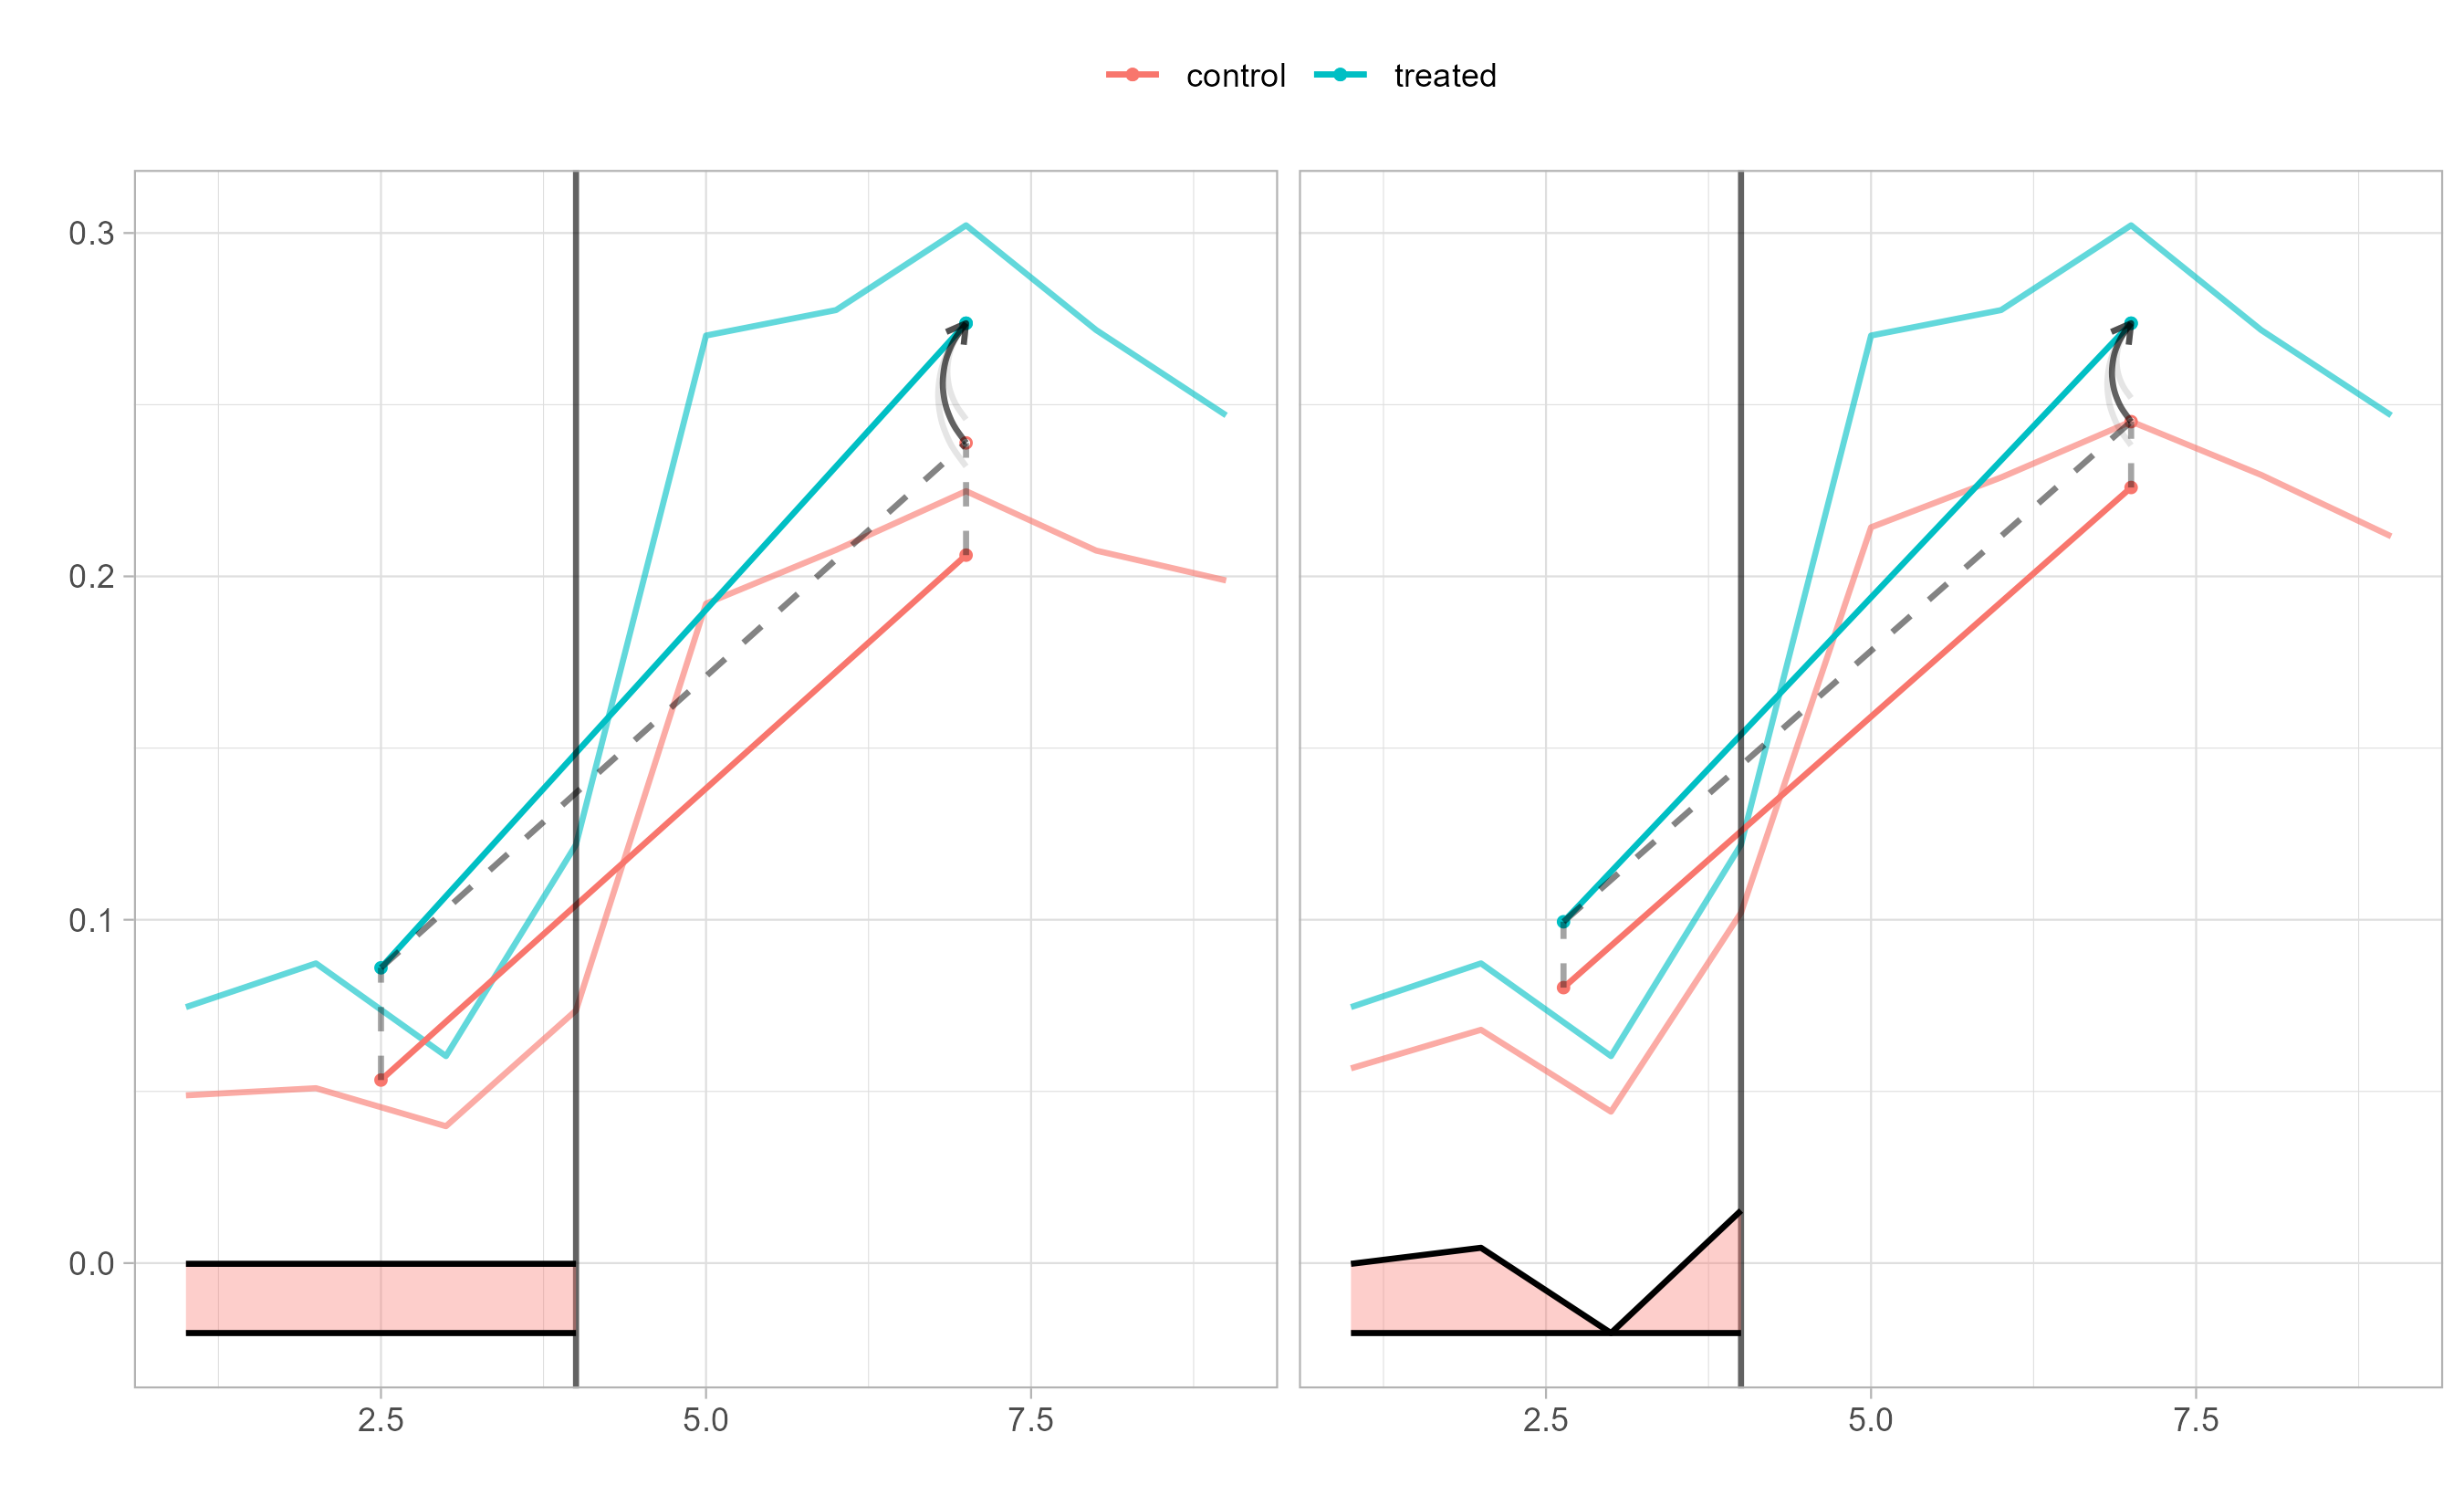
\includegraphics[width=0.7\linewidth]{../figures/results/political/comparison_pcf.png}
  \label{fig:comparison}
    \begin{minipage}{0.7\textwidth}
   \vspace{0.1in} 
   {\tiny Notes: .\par}
        \end{minipage}
\end{figure}


\begin{figure}[htbp]
  \centering
  \caption{Effect on socialist vote share - Synthetic event study}
  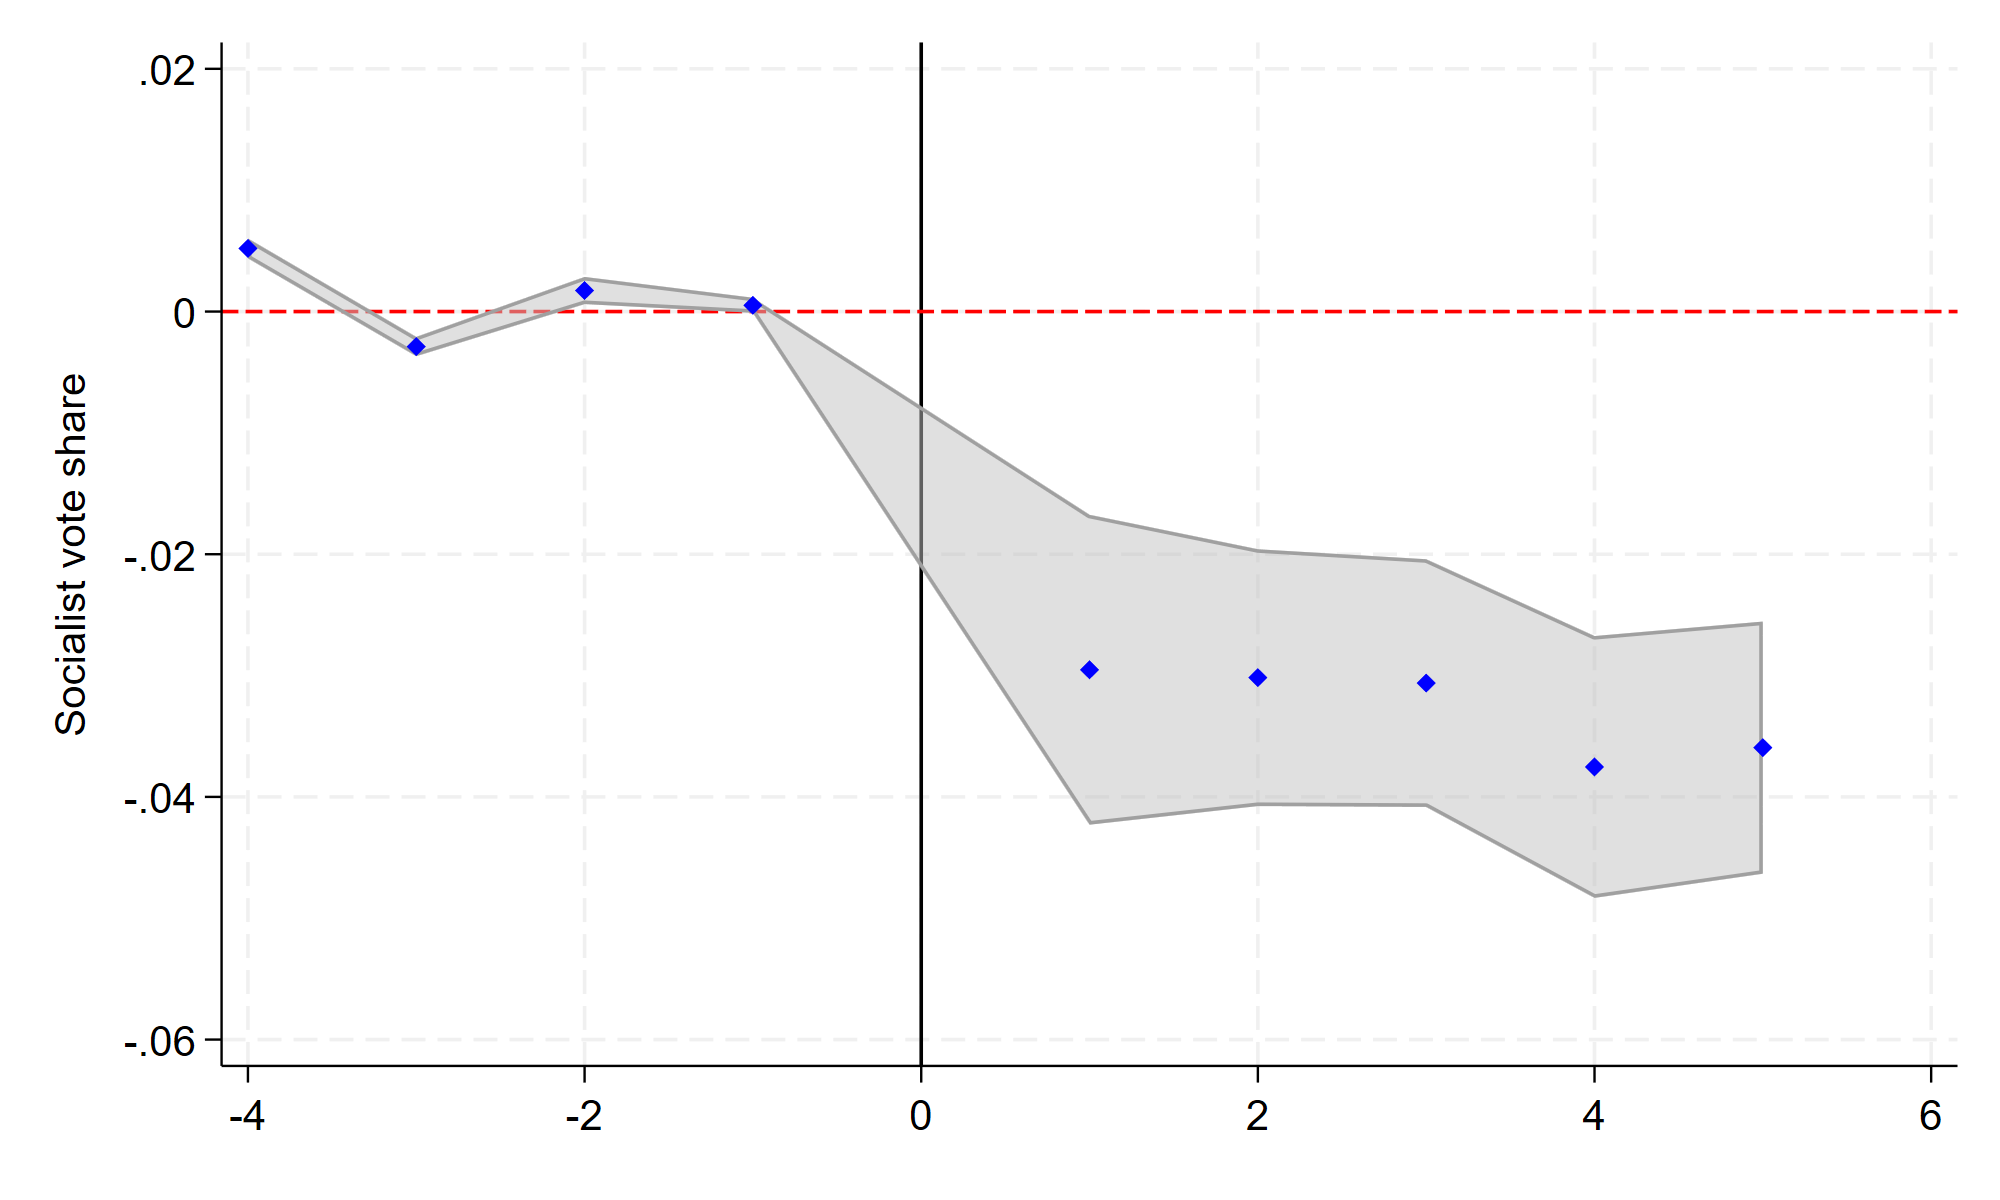
\includegraphics[width=0.7\linewidth]{../figures/results/political/sdid_event_SFIO.png}
  \label{fig:comparison}
    \begin{minipage}{0.7\textwidth}
   \vspace{0.1in} 
   {\tiny Notes: .\par}
        \end{minipage}
\end{figure}

\begin{figure}[htbp]
  \centering
  \caption{Effect on communist vote share - Synthetic event study}
  \includegraphics[width=0.7\linewidth]{../figures/results/political/sdid_event_PCF_pop.png}
  \label{fig:comparison}
    \begin{minipage}{0.7\textwidth}
   \vspace{0.1in} 
   {\tiny Notes: .\par}
        \end{minipage}
\end{figure}


CONTINUOUS DID 

The table is significant 
%\begin{table}[h!]
\centering
\caption{Impact of Camps and Refugees on Vote Shares (TWFE)}
\label{tab:twfe_camps_refugees}
\begin{tabular}{lcccc}
\hline
 & \multicolumn{2}{c}{SFIO vote share} & \multicolumn{2}{c}{PCF vote share} \\
 & (1) Camps & (2) Refugees & (3) Camps & (4) Refugees \\
\hline

Post $\times$ Camps (1 km) 
& -0.0159*** &  & 0.0115*** &  \\
 & (0.00347) &  & (0.00323) &  \\

Post $\times$ Refugees (1 km) 
&  & -3.20e-06** &  & 3.97e-07 \\
 &  & (1.11e-06) &  & (1.01e-06) \\

\hline
Observations & 74,781 & 74,781 & 74,781 & 74,781 \\
Municipality FE & Yes & Yes & Yes & Yes \\
Year $\times$ Arrondissement FE & Yes & Yes & Yes & Yes \\
\hline
\multicolumn{5}{l}{\footnotesize Standard errors clustered at the municipality level in parentheses.} \\
\multicolumn{5}{l}{\footnotesize *** $p<0.01$, ** $p<0.05$, * $p<0.1$.}
\end{tabular}
\end{table} % file not yet available

\begin{figure}[htbp]
  \centering
  \caption{Effect on socialist vote share - Continous DiD}
  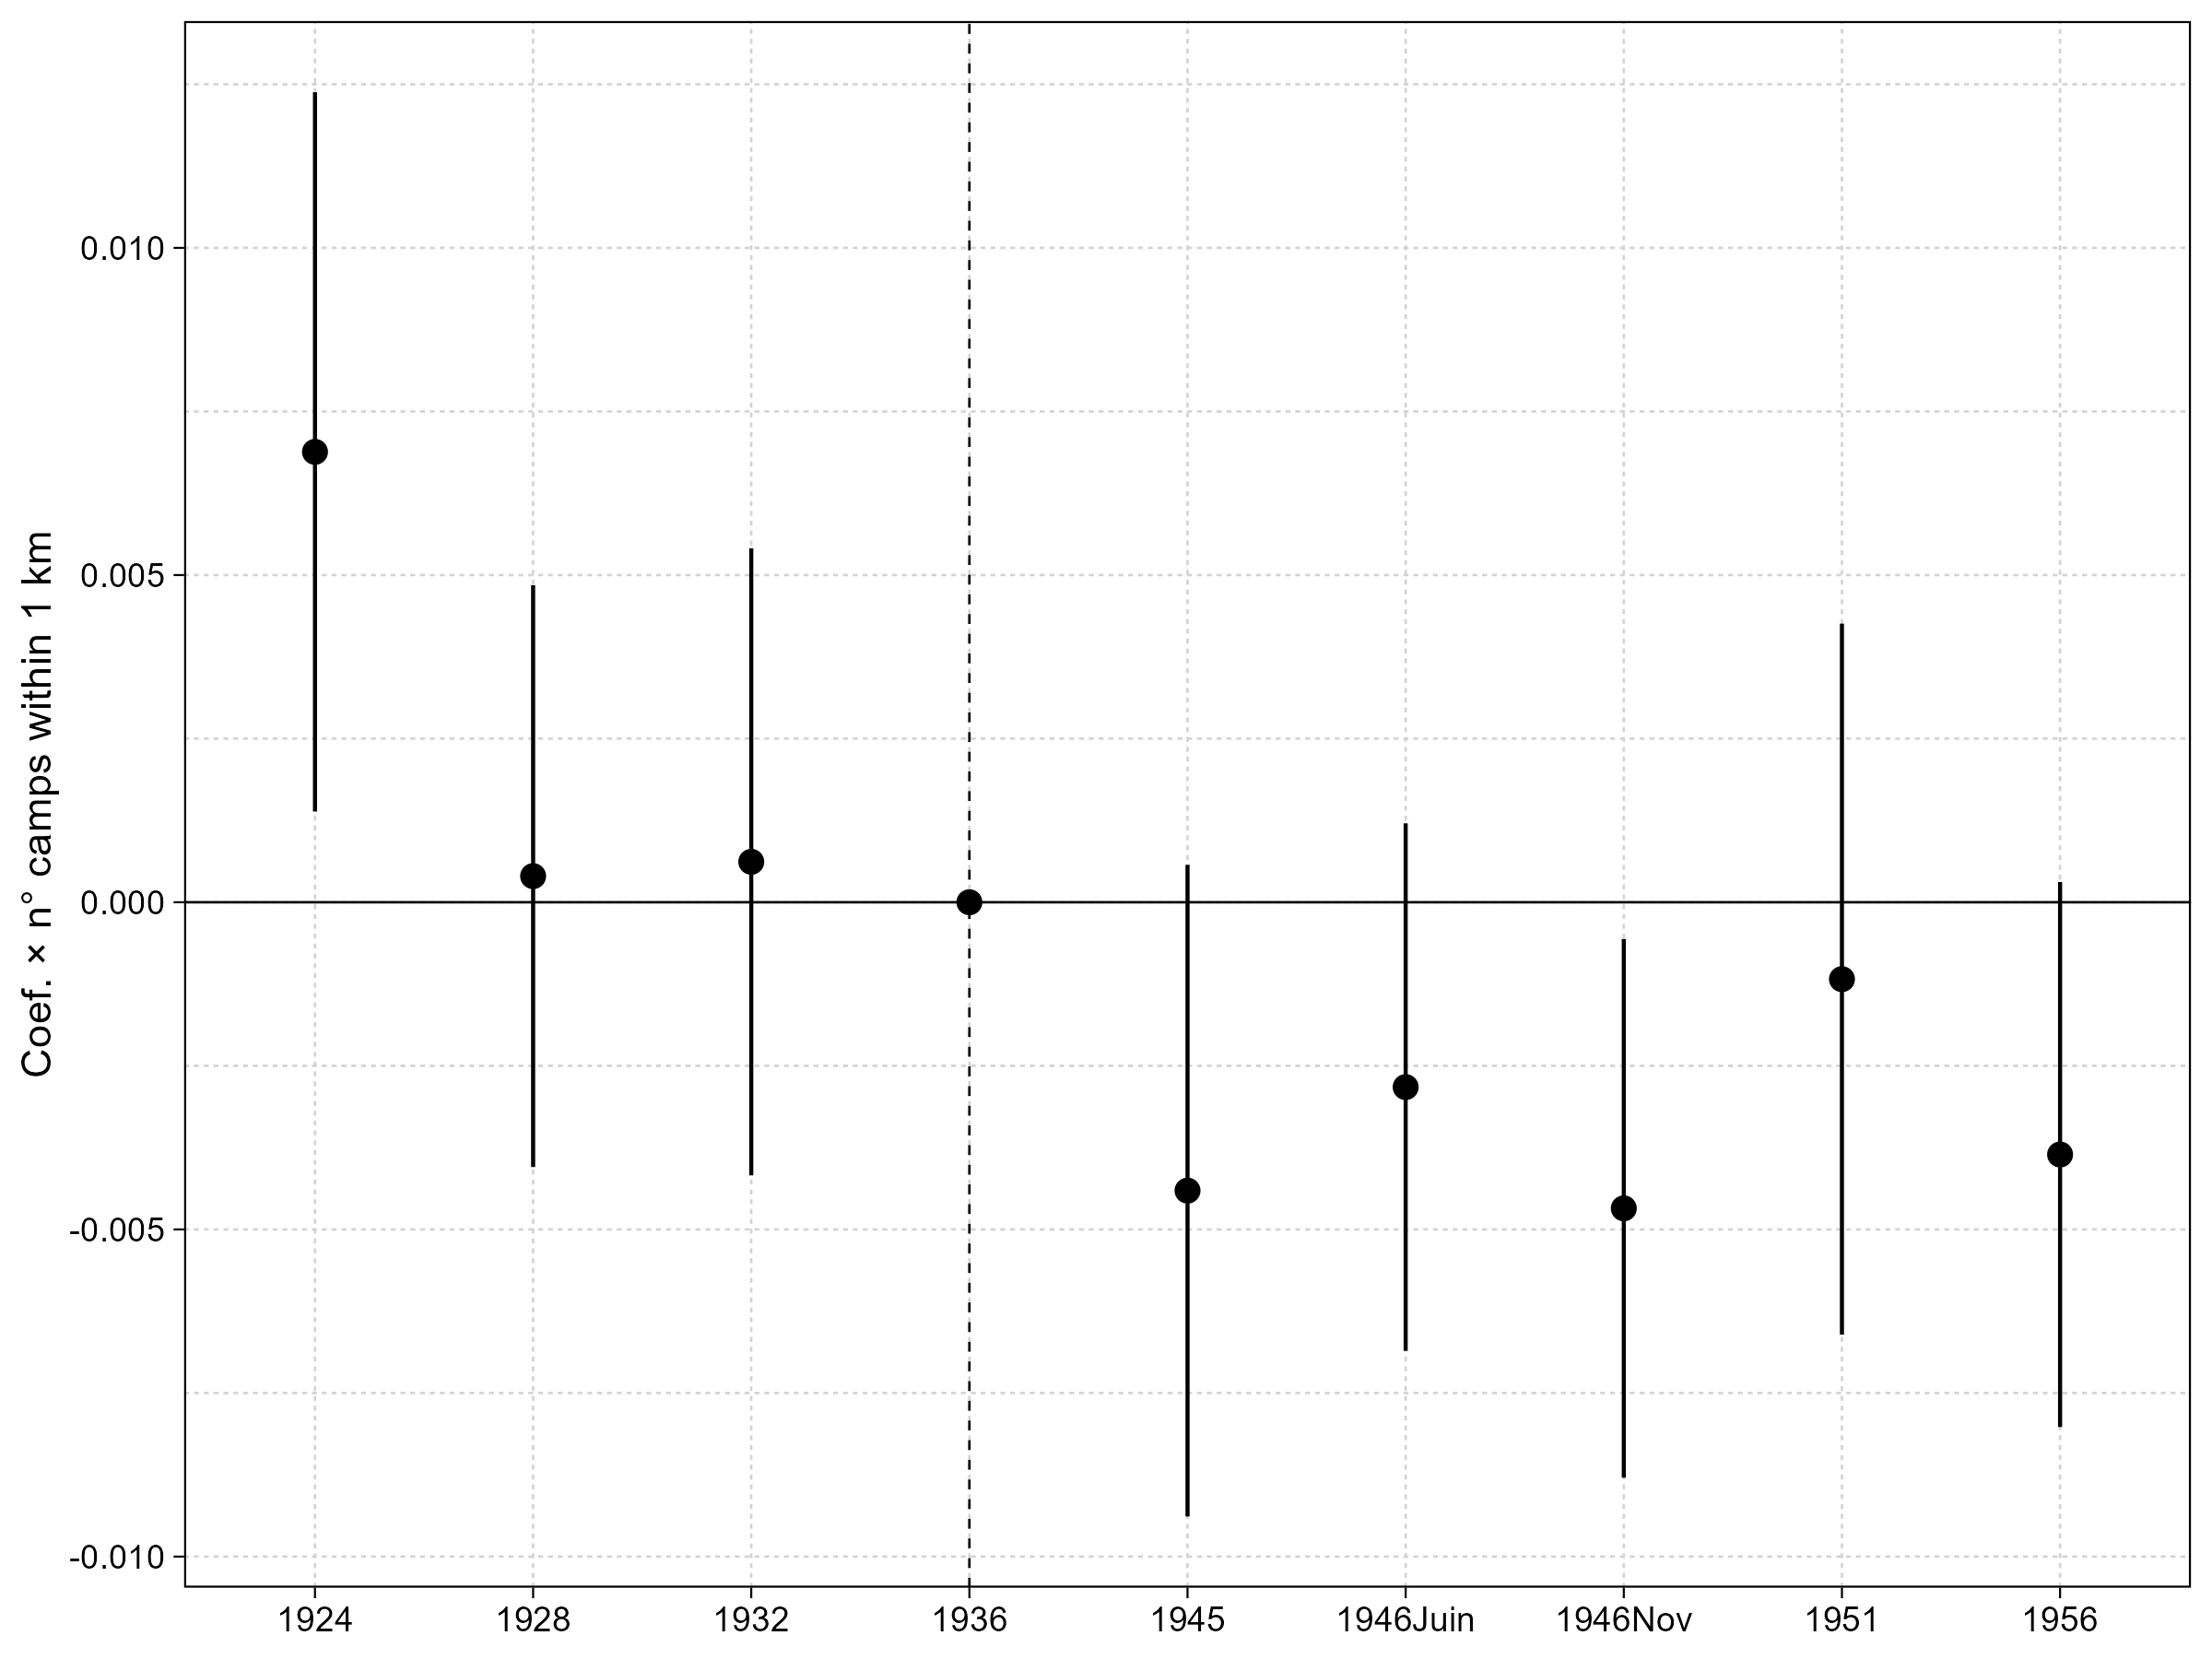
\includegraphics[width=0.7\linewidth]{../figures/results/political/cont_es_sfio_camps.png}
  \label{fig:comparison}
    \begin{minipage}{0.7\textwidth}
   \vspace{0.1in} 
   {\tiny Notes: .\par}
        \end{minipage}
\end{figure}

\begin{figure}[htbp]
  \centering
  \caption{Effect on communist vote share - Continous DiD}
  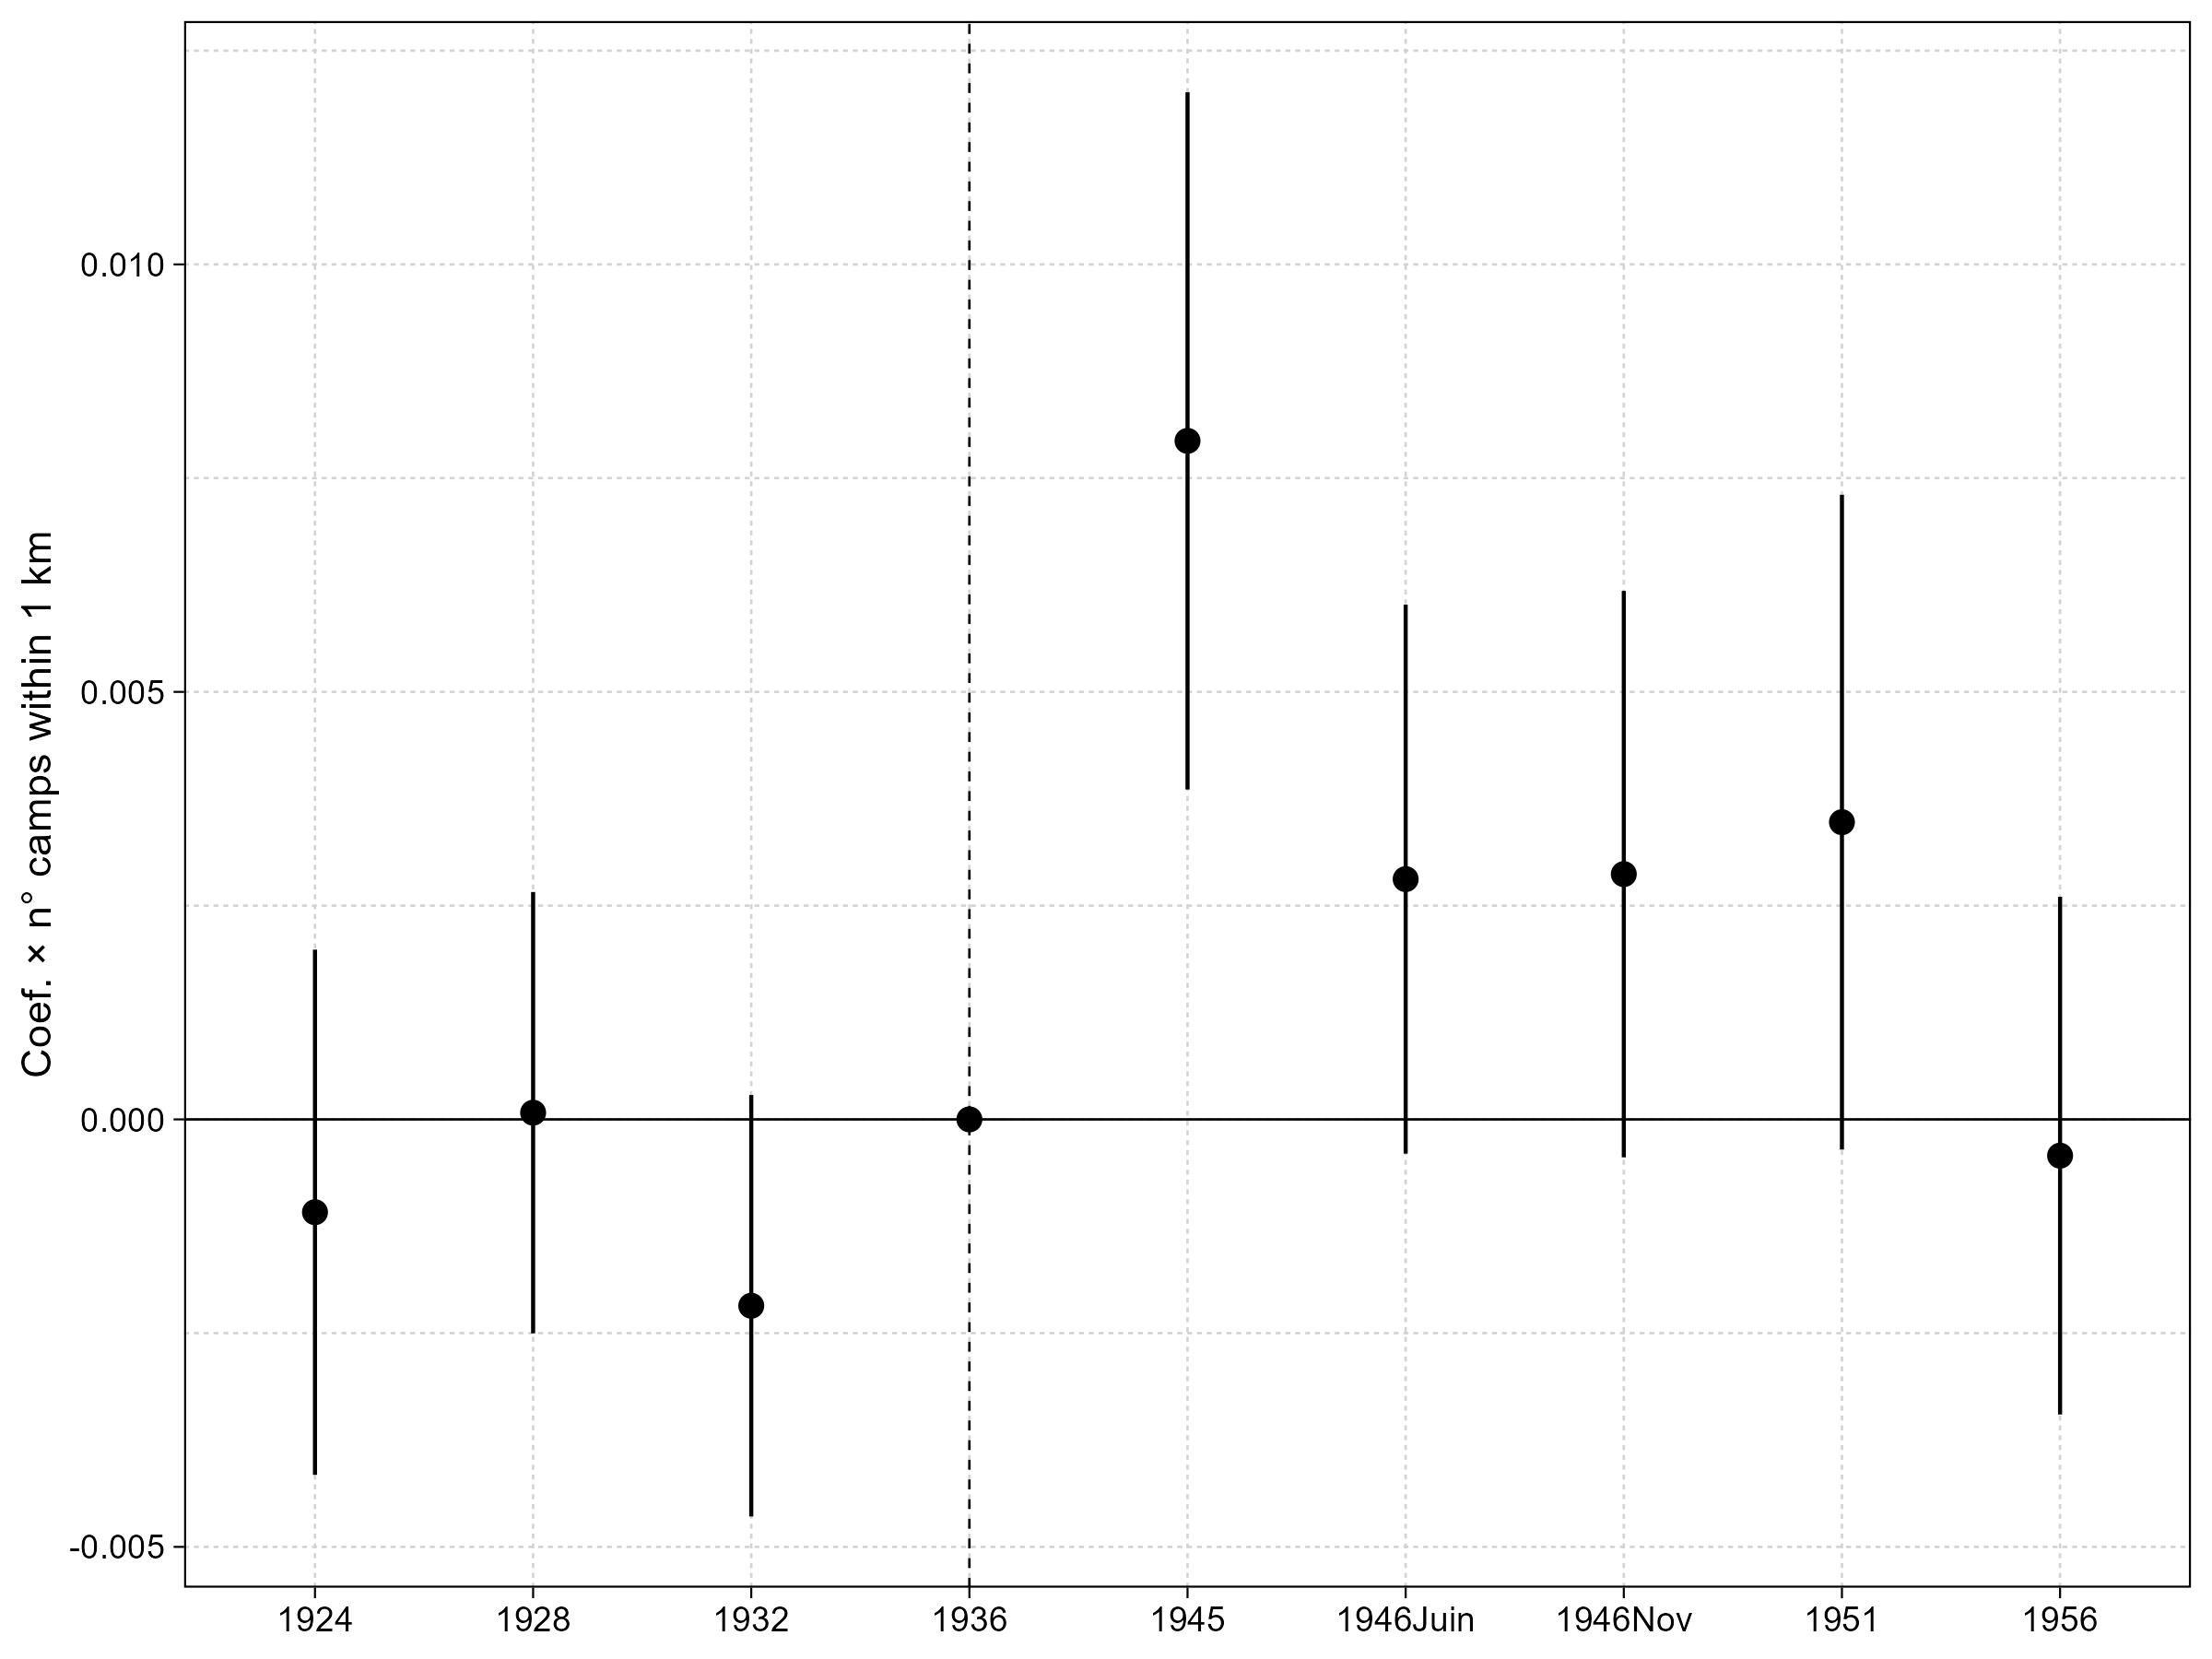
\includegraphics[width=0.7\linewidth]{../figures/results/political/cont_es_pcf_camps.png}
  \label{fig:comparison}
    \begin{minipage}{0.7\textwidth}
   \vspace{0.1in} 
   {\tiny Notes: .\par}
        \end{minipage}
\end{figure}
